\documentclass[11pt]{article}\usepackage[margin=1in]{geometry}\usepackage{amsmath,amssymb,amsthm,mathtools}\usepackage{graphicx}\graphicspath{{figures/}{../figures/}{figs/}{./}}\usepackage{enumitem}\usepackage{hyperref}\usepackage{cleveref}\usepackage{tikz}\usetikzlibrary{arrows.meta,positioning,calc,shapes.geometric}\usepackage{float}\usepackage[most]{tcolorbox}\usepackage{kotex}\usepackage{booktabs}\emergencystretch=1.6em\tolerance=2000 \crefname{assumption}{Assumption}{Assumptions}\Crefname{assumption}{Assumption}{Assumptions}\crefname{definition}{Definition}{Definitions}\Crefname{definition}{Definition}{Definitions}\crefname{proposition}{Proposition}{Propositions}\Crefname{proposition}{Proposition}{Propositions}\crefname{fact}{Fact}{Facts}\Crefname{fact}{Fact}{Facts} \newtheorem{assumption}{Assumption}\newtheorem{definition}{Definition}\newtheorem{lemma}{Lemma}\newtheorem{proposition}{Proposition}\newtheorem{theorem}{Theorem}\newtheorem{corollary}{Corollary}\newtheorem{fact}{Fact}\theoremstyle{remark}\newtheorem{remark}{Remark} \newcommand{\R}{\mathbb{R}}\newcommand{\U}{\mathcal U}
\newcommand{\Cset}{\mathcal C}\newcommand{\Pcl}{\mathcal P}\newcommand{\Zset}{\mathcal Z_0}\newcommand{\Xset}{\mathcal X_0}
\DeclareMathOperator{\clr}{clr}\newcommand{\norm}[1]{\lVert #1\rVert}\newcommand{\what}{\hat w}

\title{허용 오차와 양보로 결합된 policy의 제약 보장:\\ 상대 차수 1}
\author{Junhyeok Yoon}
\date{2026년 11월 12일}

\begin{document}
\maketitle

\begin{abstract}
사양 문서의 policy 구조(task policy, command interface, adaptive core)에 대해, 상대 차수 1인 plant class에서 허용 오차, state 제약, input 제약, 해의 존재와 사전 상한이 모든 weight와 모든 action 열에서 성립함을 증명한다. Plant에 대한 가정은 class 수준의 세 가지이다: input gain의 양정치성, 제약 영역에서의 drift 상한, saturation된 입력이 drift를 이긴다는 authority 조건. 보장은 한 부분에서 나오지 않는다. Core는 방향을 보존하는 saturation과 허용 오차 경계에서 커지는 feedback을 쓰고, interface는 오차의 여유에 따라 reference의 진행과 허용 오차의 수축을 늦춘다. 정규화 오차의 사전 상한은 둘이 함께 있을 때만 생기며, 학습되는 feedforward의 내용과 무관하다. 조건은 충분조건이고 상한은 보수적이다. 이어서 input gain이 isotropic이고 feedforward가 정확히 표현되는 경우에 한해, saturation이 작동하지 않는 구간에서 storage가 줄고 오차가 0으로 수렴하여 오차 여유에 의한 양보가 사라짐을 보인다. 기계 system은 속도와 위치를 합친 output으로 이 class에 들어간다. 그때 필요한 방향별 authority 조건이 7-DOF 수치에서 성립함을 확인하고, 관성 행렬을 모르는 경우의 storage 감소를 보인다. 정확히 표현되지 않는 경우의 수렴, 볼록하지 않은 위치 제약, 진행 보장은 다루지 않는다. 이 구조가 학습에 주는 이득은 학습 비교 노트에서 시험했고 지지되지 않았다.
\end{abstract}

\section{Overview}
\label{sec:overview}

\Cref{fig:chain}은 보장이 닫히는 순서이다. 초록색 단계는 plant와 core에 무관하게 interface만으로 성립하고, 주황색 단계는 class 조건을 쓴다. 마지막 단계는 \Cref{sec:storage}의 한정된 경우에만 성립한다. \Cref{thm:dir}는 넷째 단계의 authority 조건을 방향별 형태로 바꾸고, \Cref{sec:mech}는 기계 system을 이 순서에 넣는다. Drift 상한 $\bar F$는 해가 제약 집합 안에 있다고 이미 확인된 구간에서만 쓰이고, 보수성은 \Cref{lem:restore}의 하한과 여유 $m_\star$의 최악 경우 상수에서 생긴다.

\begin{figure}[H]
\centering
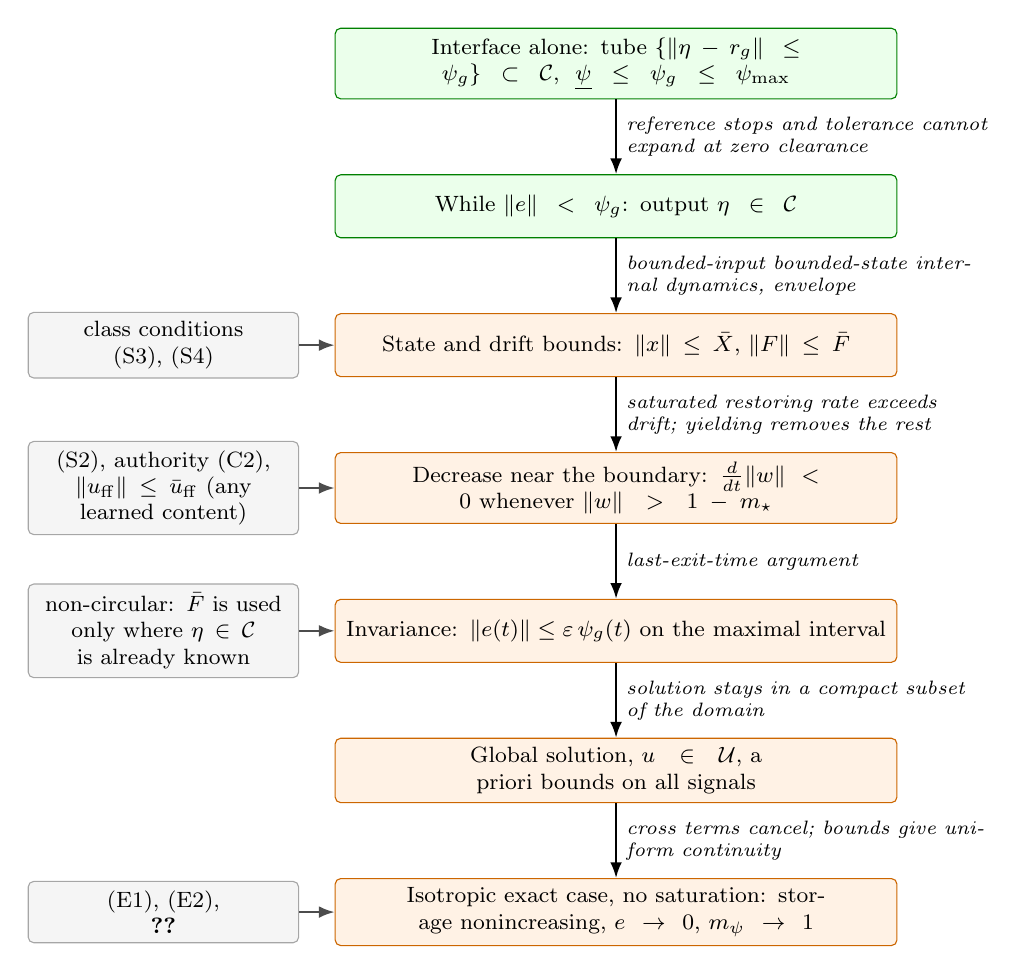
\begin{tikzpicture}[
  node distance=0.95cm and 0.45cm,
  every node/.style={font=\footnotesize, align=center},
  unc/.style={draw=green!50!black, fill=green!8, rounded corners=2pt, text width=6.9cm, minimum height=0.8cm},
  con/.style={draw=orange!80!black, fill=orange!10, rounded corners=2pt, text width=6.9cm, minimum height=0.8cm},
  feed/.style={draw=gray!70, fill=gray!8, rounded corners=2pt, text width=3.2cm, minimum height=0.75cm},
  arr/.style={-{Latex[length=2mm]}, thick},
  lab/.style={font=\scriptsize\itshape, align=left, text width=4.6cm}]
\node[unc] (n1) {Interface alone: tube $\{\|\eta-r_g\|\le\psi_g\}\subset\mathcal C$, $\ \underline\psi\le\psi_g\le\psi_{\max}$};
\node[unc, below=of n1] (n2) {While $\|e\|<\psi_g$: output $\eta\in\mathcal C$};
\node[con, below=of n2] (n3) {State and drift bounds: $\|x\|\le\bar X$, $\|F\|\le\bar F$};
\node[con, below=of n3] (n4) {Decrease near the boundary: $\tfrac{d}{dt}\|w\|<0$ whenever $\|w\|>1-m_\star$};
\node[con, below=of n4] (n5) {Invariance: $\|e(t)\|\le\varepsilon\,\psi_g(t)$ on the maximal interval};
\node[con, below=of n5] (n6) {Global solution, $u\in\mathcal U$, a priori bounds on all signals};
\node[con, below=of n6] (n7) {Isotropic exact case, no saturation: storage nonincreasing, $e\to0$, $m_\psi\to1$};
\draw[arr] (n1) -- node[lab, right]{reference stops and tolerance cannot expand at zero clearance} (n2);
\draw[arr] (n2) -- node[lab, right]{bounded-input bounded-state internal dynamics, envelope} (n3);
\draw[arr] (n3) -- node[lab, right]{saturated restoring rate exceeds drift; yielding removes the rest} (n4);
\draw[arr] (n4) -- node[lab, right]{last-exit-time argument} (n5);
\draw[arr] (n5) -- node[lab, right]{solution stays in a compact subset of the domain} (n6);
\node[feed, left=of n3] (a1) {class conditions\\ (S3), (S4)};
\node[feed, left=of n4] (a2) {(S2), authority (C2),\\ $\|u_{\mathrm{ff}}\|\le\bar u_{\mathrm{ff}}$ (any learned content)};
\draw[arr, gray!60!black] (a1) -- (n3);
\draw[arr, gray!60!black] (a2) -- (n4);
\node[feed, left=of n5] (a3) {non-circular: $\bar F$ is used only where $\eta\in\mathcal C$ is already known};
\draw[arr, gray!60!black] (a3) -- (n5);
\draw[arr] (n6) -- node[lab, right]{cross terms cancel; bounds give uniform continuity} (n7);
\node[feed, left=of n7] (a4) {(E1), (E2),\\ \Cref{prop:storage}};
\draw[arr, gray!60!black] (a4) -- (n7);
\end{tikzpicture}
\caption{Closure order of the guarantees for relative degree one}
\label{fig:chain}
\end{figure}

\section{Setting}
\label{sec:setting}

\begin{definition}[Plant class of relative degree one]
\label{def:plant}
The class $\Pcl_1$ consists of the systems
\begin{equation}
\dot x=f(x,\theta)+g_0(x)\,\Lambda(x,\theta)\,\big(u+d(x,\theta,t)\big),\qquad \eta:=c(x)\in\R^m,
\label{eq:plant}
\end{equation}
with state $x\in\R^n$, input $u\in\R^m$ and parameter $\theta$ in a given set $\Theta$, whose output satisfies
\begin{equation}
\dot\eta=F(x,\theta,t)+\Gamma(x,\theta)\,u,\qquad \Gamma:=\tfrac{\partial c}{\partial x}\,g_0\,\Lambda\in\R^{m\times m},\qquad F:=\tfrac{\partial c}{\partial x}\,f+\Gamma\,d\in\R^m,
\label{eq:output}
\end{equation}
and that satisfy, for a compact set $\Cset\subset\R^m$ (\Cref{def:constraints}), a set $\Xset\subset\R^n$ of initial states and the input set $\U$:
\begin{itemize}
\item[\textbf{(S1)}] (Measured state, regularity) $x$ is measured; $g_0$ and $c$ are known; $f$, $\Lambda$, $d$, $\theta$ are unknown; $f$, $g_0$, $\Lambda$, $d$ are locally Lipschitz in $x$, and $d$ is measurable and bounded in $t$.
\item[\textbf{(S2)}] (Input gain) $\exists$ known constants $0<\gamma_0\le\gamma_1$ such that, $\forall\,(x,\theta)$ with $c(x)\in\Cset$ and $\forall\,w\in\R^m$,
\[
w^\top\Gamma(x,\theta)\,w\ \ge\ \gamma_0\norm{w}^2,\qquad \norm{\Gamma(x,\theta)}\le\gamma_1 .
\]
\item[\textbf{(S3)}] (Internal dynamics) $\exists\,\bar X<\infty$ such that along every solution with $x(0)\in\Xset$ and $u(s)\in\U$,
\[
\eta(s)\in\Cset\ \ \forall s\in[0,t]\ \Longrightarrow\ \norm{x(t)}\le\bar X .
\]
\item[\textbf{(S4)}] (Envelope) $\exists$ a known constant $\bar F\ge0$ such that $\norm{F(x,\theta,t)}\le\bar F$ $\ \forall\,(x,\theta,t)$ with $c(x)\in\Cset$, $\norm{x}\le\bar X$, $\theta\in\Theta$, $t\ge0$.
\end{itemize}
\end{definition}

\begin{definition}[Constraints, clearance and saturation]
\label{def:constraints}
\begin{itemize}
\item State constraint: $\Cset\subset\R^m$ compact with nonempty interior.
\item Input constraint: $\U:=\{u\in\R^m:\ |u_i|\le\bar u_i,\ i=1,\dots,m\}$ with known $\bar u_i>0$; $\ \bar u_{\min}:=\min_i\bar u_i$.
\item Clearance: $\clr(r):=\inf\{\norm{r-y}:\ y\in\R^m\setminus\Cset\}$ for $r\in\R^m$.
\item Gauge of $\U$: $|v|_{\U}:=\max_i|v_i|/\bar u_i$ for $v\in\R^m$.
\item \textbf{\emph{Direction-preserving}} saturation and its factor:
\[
\sigma(v):=\lambda(v)\,v,\qquad \lambda(v):=\frac{1}{\max\{1,|v|_{\U}\}}\in(0,1].
\]
\end{itemize}
\end{definition}

\begin{fact}[Properties of the clearance and the saturation]
\label{fact:clr}
\begin{enumerate}[label=(\alph*)]
\item $\clr$ is 1-Lipschitz, and $\clr(r)\ge\psi>0\ \Rightarrow\ \{\eta:\norm{\eta-r}\le\psi\}\subset\Cset$.
\item $\sigma(v)\in\U$ $\ \forall v$; $\ \sigma(v)=v\iff v\in\U$; $\ \sigma$ is globally Lipschitz.
\end{enumerate}
\end{fact}

\begin{proof}
(a) 두 점 $r,r'$와 $y\notin\Cset$에 대해 삼각 부등식을 쓴다.
\[
\clr(r)\le\norm{r-y}\le\norm{r-r'}+\norm{r'-y}.
\]
\[
\Longrightarrow\quad \clr(r)-\clr(r')\le\norm{r-r'}.
\]
$\R^m\setminus\Cset$는 열린 집합이므로 $y\notin\Cset$, $y\ne r$이면 선분 위에 $r$에 더 가까운 $y'\notin\Cset$가 있다.
\[
y\notin\Cset\ \Longrightarrow\ \norm{r-y}>\clr(r)\ge\psi .
\]
(b) $|\sigma(v)|_{\U}=\lambda(v)|v|_{\U}\le1$이다. $|\cdot|_{\U}$는 norm이고 $\sigma$는 그 단위 공으로의 radial retraction이므로 이 norm에 대해 2-Lipschitz이다.
\end{proof}

\begin{definition}[Command, error and core]
\label{def:core}
Let $r_g(t)\in\R^m$ (realized reference) and $\psi_g(t)>0$ (realized tolerance) be absolutely continuous.
\begin{itemize}
\item Error, normalized error and transformed error, on $\{\norm{e}<\psi_g\}$:
\[
e:=\eta-r_g,\qquad w:=\frac{e}{\psi_g},\qquad \xi:=\frac{e}{\psi_g^2-\norm{e}^2}=\frac{w}{\psi_g\,(1-\norm{w}^2)} .
\]
\item Core input:
\begin{equation}
v:=u_{\mathrm{ff}}-\kappa\,\xi,\qquad u:=\sigma(v),
\label{eq:core}
\end{equation}
with feedforward $u_{\mathrm{ff}}\in\R^m$ and scalar gain $\kappa>0$.
\item Learned part: a state $z\in\R^{n_z}$ (fast weights) and maps
\[
\dot z=Z(t,x,r_g,\psi_g,z),\qquad u_{\mathrm{ff}}=U_{\mathrm{ff}}(t,x,r_g,\psi_g,z),\qquad \kappa=K(t,x,r_g,\psi_g,z),
\]
that satisfy, for design constants $\bar u_{\mathrm{ff}}\ge0$, $0<\kappa_0\le\kappa_1$ and a compact set $\Zset\subset\R^{n_z}$:
\begin{itemize}
\item[\textbf{(F1)}] $\norm{U_{\mathrm{ff}}}\le\bar u_{\mathrm{ff}}$ and $\kappa_0\le K\le\kappa_1$ everywhere;
\item[\textbf{(F2)}] $Z$, $U_{\mathrm{ff}}$, $K$ are locally Lipschitz in $(x,r_g,\psi_g,z)$ and measurable in $t$;
\item[\textbf{(F3)}] $\Zset$ is forward invariant for $\dot z=Z$ under every input signal.
\end{itemize}
\end{itemize}
\end{definition}

\begin{definition}[Proposal and command interface]
\label{def:interface}
\begin{itemize}
\item Proposal: measurable $v_p(t)\in\R^m$ with $\norm{v_p}\le\bar v$ and $\psi_p(t)\in[\underline\psi,\bar\psi]$, $0<\underline\psi\le\bar\psi$.
\item Margins, with a design constant $c_0>0$:
\[
m_\psi:=1-\norm{w},\qquad m_{\Cset}:=\min\Big\{1,\ \max\Big\{0,\ \frac{\clr(r_g)-\psi_g}{c_0}\Big\}\Big\} .
\]
\item \textbf{\emph{Yield functions}}: $\gamma_r,\gamma_\psi,\gamma_+:[0,1]\to[0,1]$, Lipschitz, nondecreasing, with $\gamma_r(0)=\gamma_\psi(0)=\gamma_+(0)=0$.
\item Interface, with a design constant $\alpha>0$ and $(\cdot)^+:=\max\{\cdot,0\}$:
\begin{align}
\dot r_g&=\gamma_r\big(\min\{m_\psi,m_{\Cset}\}\big)\,v_p, \label{eq:rg}\\
\dot\psi_g&=-\alpha\,\gamma_\psi(m_\psi)\,(\psi_g-\psi_p)^+ +\alpha\,\gamma_+(m_{\Cset})\,(\psi_p-\psi_g)^+ . \label{eq:psig}
\end{align}
\end{itemize}
\end{definition}

\begin{assumption}[Admissibility]
\label{ass:adm}
\begin{itemize}
\item[\textbf{(C1)}] (Initial condition) $x(0)\in\Xset$, $z(0)\in\Zset$, $\ \norm{e(0)}<\psi_g(0)$, $\ \psi_g(0)\ge\underline\psi$, $\ \clr(r_g(0))\ge\psi_g(0)$.
\item[\textbf{(C2)}] (Authority) $\rho_0:=\gamma_0\,\bar u_{\min}-\bar F>0$.
\end{itemize}
\end{assumption}

\begin{definition}[A priori margin]
\label{def:margin}
Let $\psi_{\max}:=\max\{\psi_g(0),\bar\psi\}$. For $s\ge0$ and $m\in(0,1)$ define
\begin{align}
\Psi(s)&:=\min\Big\{1,\ \frac{\bar u_{\min}}{\bar u_{\mathrm{ff}}+s}\Big\}\,\big(\gamma_0\,s-\gamma_1\,\bar u_{\mathrm{ff}}\big), \label{eq:Psi}\\
s_{\mathrm{low}}(m)&:=\frac{\kappa_0\,(1-m)}{\psi_{\max}\,m\,(2-m)}, \label{eq:slow}\\
\Phi(m)&:=\gamma_r(m)\,\bar v+\alpha\,\gamma_\psi(m)\,(\psi_{\max}-\underline\psi)+\gamma_0\,\bar u_{\min}-\Psi\big(s_{\mathrm{low}}(m)\big). \label{eq:Phi}
\end{align}
The \textbf{\emph{a priori margin}} is
\[
m_\star:=\sup\Big\{\mu\in(0,1):\ \Phi(m)<\rho_0\ \text{ and }\ s_{\mathrm{low}}(m)\ge\frac{\gamma_1\bar u_{\mathrm{ff}}}{\gamma_0}\quad\forall m\in(0,\mu]\Big\}.
\]
\end{definition}

\section{Constraint guarantee}
\label{sec:result}

\textbf{직관 (두 종류의 양보).} 입력에 상한이 있으면 경계에서 커지는 feedback만으로는 오차를 허용 오차 안에 둘 수 없다. Reference가 plant가 따라갈 수 있는 것보다 빨리 움직이면 입력은 이미 한계에 있으므로 오차가 경계에 닿는다. 입력 제약을 다루는 기존 funnel 제어는 이때 경계를 넓혀 보장을 유지하지만, 넓어지는 양에 상한이 없어서 고정된 state 제약과 양립하지 않는다(\Cref{sec:comp}). 여기서는 위층이 양보한다. 오차가 경계에 가까워질수록 interface가 reference의 진행과 허용 오차의 수축을 늦추고, 경계에서는 둘 다 멈춘다. 그러면 경계 근처에서 오차를 키우는 것은 plant의 drift뿐이고, authority 조건 (C2)는 saturation된 입력이 그 drift를 이긴다는 조건이다. 이 논증은 saturation이 입력의 방향을 바꾸지 않는다는 점에 의존한다. 대가는 진행 속도이다. 보장은 제안된 명령이 아니라 실현된 명령에 대해 성립하고, 둘의 차이는 아래층이 지금 무엇을 할 수 있는지의 측정값이 된다.

\begin{lemma}[Restoring rate of the saturated input]
\label{lem:restore}
Let $\Gamma\in\R^{m\times m}$ satisfy the two inequalities of (S2). Then, $\forall\,\what\in\R^m$ with $\norm{\what}=1$, $\forall\,u_{\mathrm{ff}}\in\R^m$ with $\norm{u_{\mathrm{ff}}}\le\bar u_{\mathrm{ff}}$ and $\forall\,s\ge\gamma_1\bar u_{\mathrm{ff}}/\gamma_0$,
\[
\what^\top\Gamma\,\sigma(u_{\mathrm{ff}}-s\,\what)\ \le\ -\Psi(s),
\]
and $\Psi$ is nondecreasing on $[\gamma_1\bar u_{\mathrm{ff}}/\gamma_0,\infty)$ with $\ \lim_{s\to\infty}\Psi(s)=\gamma_0\,\bar u_{\min}$.
\end{lemma}

\begin{proof}
$v:=u_{\mathrm{ff}}-s\what$, $\lambda:=\lambda(v)$로 둔다. (S2)를 쓴다.
\[
\what^\top\Gamma\,\sigma(v)=\lambda\,\what^\top\Gamma u_{\mathrm{ff}}-\lambda\,s\,\what^\top\Gamma\what\ \le\ -\lambda\,(\gamma_0 s-\gamma_1\bar u_{\mathrm{ff}}).
\]
Gauge를 Euclidean norm으로 누른다.
\[
|v|_{\U}\le\frac{\norm{v}_\infty}{\bar u_{\min}}\le\frac{\bar u_{\mathrm{ff}}+s}{\bar u_{\min}}
\]
\[
\Longrightarrow\quad \lambda\ \ge\ \min\Big\{1,\ \frac{\bar u_{\min}}{\bar u_{\mathrm{ff}}+s}\Big\}.
\]
$\gamma_0s-\gamma_1\bar u_{\mathrm{ff}}\ge0$이므로 $\lambda$의 하한을 대입하면 첫 주장이 나온다. 단조성은 두 구간에서 미분으로 확인한다.
\[
\frac{d}{ds}\Psi(s)=
\begin{cases}
\gamma_0, & \bar u_{\mathrm{ff}}+s\le\bar u_{\min},\\[2pt]
\dfrac{\bar u_{\min}\,(\gamma_0+\gamma_1)\,\bar u_{\mathrm{ff}}}{(\bar u_{\mathrm{ff}}+s)^2}, & \bar u_{\mathrm{ff}}+s>\bar u_{\min}.
\end{cases}
\]
\end{proof}

\begin{lemma}[Tube inside the constraint set]
\label{lem:tube}
Let $(r_g,\psi_g)$ solve \eqref{eq:rg}--\eqref{eq:psig} on $[0,\omega)$, $\omega\in(0,\infty]$, for an arbitrary measurable proposal and an arbitrary measurable signal $m_\psi(t)\in[0,1]$, with $\psi_g(0)\ge\underline\psi$ and $\clr(r_g(0))\ge\psi_g(0)$. Then, $\forall t\in[0,\omega)$,
\begin{enumerate}[label=(\alph*)]
\item $\underline\psi\le\psi_g(t)\le\psi_{\max}$;
\item $\clr(r_g(t))\ge\psi_g(t)$.
\end{enumerate}
\end{lemma}

\begin{proof}
(a) $\psi_p\in[\underline\psi,\bar\psi]$이므로 \eqref{eq:psig}의 부호가 구간 밖에서 정해진다.
\[
\psi_g>\bar\psi\ \Rightarrow\ \dot\psi_g\le0,\qquad \psi_g<\underline\psi\ \Rightarrow\ \dot\psi_g\ge0 .
\]
(b) $D:=\clr(r_g)-\psi_g$는 \Cref{fact:clr}(a)에 의해 절대 연속이다. $D(t_1)<0$인 $t_1$이 있다고 하고 마지막 영점을 잡는다.
\[
t_0:=\sup\{t<t_1:\ D(t)\ge0\},\qquad D(t_0)=0,\qquad D<0\ \text{ on }(t_0,t_1].
\]
그 구간에서 $m_{\Cset}=0$이므로 reference가 멈추고 확장 항이 사라진다.
\[
\dot r_g=0,\qquad \dot\psi_g=-\alpha\,\gamma_\psi(m_\psi)\,(\psi_g-\psi_p)^+\le0 .
\]
\[
\Longrightarrow\quad \dot D=-\dot\psi_g\ge0\ \text{ a.e. on }(t_0,t_1]\ \Longrightarrow\ D(t_1)\ge D(t_0)=0 ,
\]
이는 $D(t_1)<0$과 모순이다.
\end{proof}

\begin{theorem}[Constraint guarantee for relative degree one]
\label{thm:main}
Consider a plant in $\Pcl_1$, the core of \Cref{def:core} with any learned part satisfying (F1)--(F3), and the interface of \Cref{def:interface}, under \Cref{ass:adm}. Then $m_\star>0$, and for every $\theta\in\Theta$, every proposal and every initial condition satisfying (C1), the closed loop has a unique solution on $[0,\infty)$ which satisfies, $\forall t\ge0$:
\begin{enumerate}[label=(\alph*)]
\item (Tolerance) $\norm{e(t)}\le\varepsilon\,\psi_g(t)$ with $\ \varepsilon:=\max\big\{\norm{e(0)}/\psi_g(0),\ 1-m_\star\big\}<1$;
\item (State constraint) $\eta(t)\in\Cset$;
\item (Input constraint) $u(t)\in\U$;
\item (A priori bounds) $\underline\psi\le\psi_g(t)\le\psi_{\max}$, $\ \clr(r_g(t))\ge\psi_g(t)$, $\ z(t)\in\Zset$, $\ \norm{x(t)}\le\bar X$, and
\[
\norm{\xi(t)}\le\frac{\varepsilon}{\underline\psi\,(1-\varepsilon^2)},\qquad \norm{v(t)}\le\bar u_{\mathrm{ff}}+\frac{\kappa_1\,\varepsilon}{\underline\psi\,(1-\varepsilon^2)} .
\]
\end{enumerate}
The condition (C2) is sufficient, not necessary, and the bound $\varepsilon$ is conservative.
\end{theorem}

\begin{proof}
\textbf{Step 1 (여유의 존재).} $m\to0^+$에서 $s_{\mathrm{low}}(m)\to\infty$이고 yield function은 0에서 0이다. \Cref{lem:restore}의 극한을 쓴다.
\[
\lim_{m\to0^+}\Phi(m)=\gamma_0\bar u_{\min}-\lim_{s\to\infty}\Psi(s)=0<\rho_0
\]
\[
\Longrightarrow\quad m_\star>0 .
\]
$\Phi$는 $m$에 대해 비감소이다. $\gamma_r,\gamma_\psi$는 비감소, $s_{\mathrm{low}}$는 감소, $\Psi$는 비감소이기 때문이다.

\textbf{Step 2 (최대 해).} Closed-loop 상태를 $\zeta:=(x,z,r_g,\psi_g)$로 두고 정의역을 연다.
\[
\mathcal D:=\{\zeta:\ \norm{c(x)-r_g}<\psi_g,\ \psi_g>0\}.
\]
(S1), (F2), \Cref{fact:clr}에 의해 우변은 $\mathcal D$에서 $\zeta$에 대해 locally Lipschitz이고 $t$에 대해 measurable이다. 따라서 유일한 최대 해가 $[0,\omega)$에 존재하고, $\omega<\infty$이면 해는 $\mathcal D$의 모든 compact 부분집합을 벗어난다.

\textbf{Step 3 (제약 집합 안의 output).} \Cref{lem:tube}와 $\norm{e}<\psi_g$를 합친다.
\[
\norm{\eta(t)-r_g(t)}<\psi_g(t)\le\clr(r_g(t))\qquad\forall t\in[0,\omega)
\]
\[
\Longrightarrow\quad \eta(t)\in\Cset\qquad\forall t\in[0,\omega).
\]
\eqref{eq:core}에 의해 $u\in\U$이므로 (S3), (S4)가 적용된다.
\[
\norm{x(t)}\le\bar X,\qquad \norm{F(x(t),\theta,t)}\le\bar F\qquad\forall t\in[0,\omega).
\]

\textbf{Step 4 (경계 근처의 감소).} $e\ne0$에서 $\what:=e/\norm{e}$로 두면 \eqref{eq:output}에서 다음을 얻는다.
\[
\frac{d}{dt}\norm{e}=\what^\top\big(F+\Gamma\,\sigma(u_{\mathrm{ff}}-s\,\what)-\dot r_g\big),\qquad s:=\kappa\,\norm{\xi}=\frac{\kappa\,\norm{w}}{\psi_g\,(1-\norm{w}^2)} .
\]
\[
\frac{d}{dt}\norm{w}=\frac{1}{\psi_g}\Big(\frac{d}{dt}\norm{e}-\norm{w}\,\dot\psi_g\Big).
\]
Interface의 두 항을 yield function으로 누른다.
\[
-\what^\top\dot r_g\le\gamma_r(m_\psi)\,\bar v,\qquad -\norm{w}\,\dot\psi_g\le\alpha\,\gamma_\psi(m_\psi)\,(\psi_{\max}-\underline\psi).
\]
$m_\psi<m_\star$인 점에서 $1-\norm{w}^2=m_\psi(2-m_\psi)$와 (F1)을 쓴다.
\[
s\ \ge\ s_{\mathrm{low}}(m_\psi)\ \ge\ \frac{\gamma_1\bar u_{\mathrm{ff}}}{\gamma_0}.
\]
\Cref{lem:restore}와 $\Psi$의 단조성을 쓴다.
\[
\what^\top\Gamma\,\sigma(u_{\mathrm{ff}}-s\,\what)\le-\Psi(s)\le-\Psi\big(s_{\mathrm{low}}(m_\psi)\big).
\]
세 부등식과 Step 3의 $\norm{F}\le\bar F$를 더한다.
\[
\psi_g\,\frac{d}{dt}\norm{w}\ \le\ \Phi(m_\psi)-\rho_0\ <\ 0\qquad\text{a.e. on }\{t\in[0,\omega):\ \norm{w(t)}>1-m_\star\}.
\]

\textbf{Step 5 (불변성).} $\norm{w(t_1)}>\varepsilon$인 $t_1\in[0,\omega)$가 있다고 하고 마지막 통과 시각을 잡는다.
\[
t_0:=\max\{t\in[0,t_1):\ \norm{w(t)}=\varepsilon\},\qquad \norm{w}>\varepsilon\ge1-m_\star\ \text{ on }(t_0,t_1].
\]
Step 4를 적분한다.
\[
\norm{w(t_1)}\le\norm{w(t_0)}=\varepsilon ,
\]
이는 모순이다.
\[
\Longrightarrow\quad \norm{e(t)}\le\varepsilon\,\psi_g(t)\qquad\forall t\in[0,\omega).
\]

\textbf{Step 6 (전역 존재).} Step 3, Step 5, \Cref{lem:tube}, (F3)에 의해 해는 다음 집합에 머문다.
\[
\mathcal K:=\big\{\zeta:\ \norm{x}\le\bar X,\ z\in\Zset,\ \clr(r_g)\ge\psi_g,\ \underline\psi\le\psi_g\le\psi_{\max},\ \norm{c(x)-r_g}\le\varepsilon\,\psi_g\big\}.
\]
$\clr(r_g)\ge\underline\psi>0$이면 $r_g\in\Cset$이므로 $\mathcal K$는 $\mathcal D$의 compact 부분집합이다.
\[
\Longrightarrow\quad \omega=\infty .
\]

\textbf{Step 7 (나머지 상한).} (a), (b), (c)와 (d)의 앞 네 항은 Step 3, 5, 6에서 나왔다. $\xi$와 $v$의 상한은 (a)와 (F1)에서 나온다.
\[
\norm{\xi}=\frac{\norm{w}}{\psi_g\,(1-\norm{w}^2)}\le\frac{\varepsilon}{\underline\psi\,(1-\varepsilon^2)} .
\]
\end{proof}

\begin{corollary}[Independence from the learned content]
\label{cor:learn}
The constants $m_\star$ and $\varepsilon$ of \Cref{thm:main} depend only on the class data $(\gamma_0,\gamma_1,\bar u_{\min},\bar F)$, the design data $(\bar u_{\mathrm{ff}},\kappa_0,\alpha,\bar v,\underline\psi,\bar\psi,\gamma_r,\gamma_\psi)$ and the initial values $\norm{e(0)}/\psi_g(0)$, $\psi_g(0)$. Consequently, (a)--(d) hold
\begin{enumerate}[label=(\alph*)]
\item for every weight of the networks that generate $v_p$, $\psi_p$, $u_{\mathrm{ff}}$, $\kappa$ and $\dot z$;
\item under arbitrary measurable time variation of these weights;
\item for every exploration signal added to the proposal that keeps $\norm{v_p}\le\bar v$ and $\psi_p\in[\underline\psi,\bar\psi]$.
\end{enumerate}
\end{corollary}

\begin{proof}
\Cref{thm:main}의 가정에서 학습되는 부분은 (F1)--(F3)과 제안의 범위로만 나타나고, (F2)는 $t$에 대한 의존을 허용한다.
\end{proof}

\begin{definition}[Restoring function and directional authority]
\label{def:restore}
Let $\Omega$ be the set of triples $(x,\theta,t)$ with $c(x)\in\Cset$, $\norm{x}\le\bar X$, $\theta\in\Theta$, $t\ge0$, and $\sigma_\infty(v):=v/|v|_{\U}$ for $v\ne0$. For $s\ge0$,
\begin{align}
R(s)&:=\sup\Big\{\what^\top\big(F(x,\theta,t)+\Gamma(x,\theta)\,\sigma(u_{\mathrm{ff}}-s'\what)\big):\ s'\ge s,\ \norm{\what}=1,\ \norm{u_{\mathrm{ff}}}\le\bar u_{\mathrm{ff}},\ (x,\theta,t)\in\Omega\Big\}, \label{eq:R}\\
\rho_{\mathrm{dir}}&:=-\sup\Big\{\what^\top\big(F(x,\theta,t)+\Gamma(x,\theta)\,\sigma_\infty(-\what)\big):\ \norm{\what}=1,\ (x,\theta,t)\in\Omega\Big\}. \label{eq:rhodir}
\end{align}
\end{definition}

\begin{lemma}[Bounds of the restoring function]
\label{lem:Rbounds}
Let $\norm{F}\le\bar F$ and $\norm{\Gamma}\le\gamma_1$ on $\Omega$, $\bar u_{\max}:=\max_i\bar u_i$, $L_\sigma:=2\sqrt m\,\bar u_{\max}\big(1+\sqrt m\,\bar u_{\max}/\bar u_{\min}\big)$ and $s_1:=2\sqrt m\,\bar u_{\max}\max\{1,\bar u_{\mathrm{ff}}/\bar u_{\min}\}$. Then $R$ is nonincreasing and
\begin{enumerate}[label=(\alph*)]
\item $R(s)\le-\rho_{\mathrm{dir}}+\gamma_1\,L_\sigma\,\bar u_{\mathrm{ff}}/s$ $\ \forall s\ge s_1$, and $\lim_{s\to\infty}R(s)=-\rho_{\mathrm{dir}}$;
\item under (S2): $R(s)\le\bar F-\Psi(s)$ $\ \forall s\ge\gamma_1\bar u_{\mathrm{ff}}/\gamma_0$, and $\rho_{\mathrm{dir}}\ge\rho_0$.
\end{enumerate}
\end{lemma}

\begin{proof}
단조성은 \eqref{eq:R}의 $s'\ge s$에서 나온다. (a) $x:=\what-u_{\mathrm{ff}}/s$로 두면 $u_{\mathrm{ff}}-s\what=-s\,x$이다. Gauge와 norm의 관계 $\norm{z}_\infty/\bar u_{\max}\le|z|_{\U}\le\norm{z}/\bar u_{\min}$, $\norm{z}_\infty\ge\norm{z}/\sqrt m$을 쓴다.
\[
|\what|_{\U}\ge\frac{1}{\sqrt m\,\bar u_{\max}},\qquad |x|_{\U}\ge|\what|_{\U}-\frac{\bar u_{\mathrm{ff}}}{s\,\bar u_{\min}}\ge\frac{1}{2\sqrt m\,\bar u_{\max}}\qquad(s\ge s_1).
\]
$s\ge s_1$이면 $s|x|_{\U}\ge1$이므로 saturation이 작동한다.
\[
\sigma(u_{\mathrm{ff}}-s\what)=-\frac{x}{|x|_{\U}},\qquad \sigma_\infty(-\what)=-\frac{\what}{|\what|_{\U}} .
\]
두 점의 차이를 나눈다.
\[
\frac{x}{|x|_{\U}}-\frac{\what}{|\what|_{\U}}=\frac{x-\what}{|x|_{\U}}+\what\,\frac{|\what|_{\U}-|x|_{\U}}{|x|_{\U}\,|\what|_{\U}} .
\]
$\norm{x-\what}\le\bar u_{\mathrm{ff}}/s$와 $\big||\what|_{\U}-|x|_{\U}\big|\le\bar u_{\mathrm{ff}}/(s\,\bar u_{\min})$를 넣는다.
\[
\norm{\sigma(u_{\mathrm{ff}}-s\what)-\sigma_\infty(-\what)}\le\frac{L_\sigma\,\bar u_{\mathrm{ff}}}{s}
\]
\[
\Longrightarrow\quad \what^\top\big(F+\Gamma\,\sigma(u_{\mathrm{ff}}-s\what)\big)\le-\rho_{\mathrm{dir}}+\frac{\gamma_1\,L_\sigma\,\bar u_{\mathrm{ff}}}{s} .
\]
$u_{\mathrm{ff}}=0$에서는 $s'|\what|_{\U}\ge1$이면 $\sigma(-s'\what)=\sigma_\infty(-\what)$이므로 $R(s)\ge-\rho_{\mathrm{dir}}$이고, 극한이 정해진다. (b) 첫 부등식은 \Cref{lem:restore}와 $\Psi$의 단조성이다. $|\what|_{\U}\le1/\bar u_{\min}$을 쓴다.
\[
\what^\top\Gamma\,\sigma_\infty(-\what)=-\frac{\what^\top\Gamma\what}{|\what|_{\U}}\le-\gamma_0\,\bar u_{\min}\ \Longrightarrow\ \rho_{\mathrm{dir}}\ge\gamma_0\bar u_{\min}-\bar F=\rho_0 .
\]
\end{proof}

\begin{theorem}[Constraint guarantee under directional authority]
\label{thm:dir}
Let the hypotheses of \Cref{thm:main} hold with (C2) replaced by $\rho_{\mathrm{dir}}>0$, and define
\begin{align*}
\Phi_R(m)&:=\gamma_r(m)\,\bar v+\alpha\,\gamma_\psi(m)\,(\psi_{\max}-\underline\psi)+R\big(s_{\mathrm{low}}(m)\big),\\
m_\star^R&:=\sup\big\{\mu\in(0,1):\ \Phi_R(m)<0\ \ \forall m\in(0,\mu]\big\}.
\end{align*}
Then $m_\star^R>0$, and (a)--(d) of \Cref{thm:main} hold with $m_\star$ replaced by $m_\star^R$. Under (C2), $m_\star^R\ge m_\star$.
\end{theorem}

\begin{proof}
$R$은 비증가이고 $s_{\mathrm{low}}$는 감소하므로 $\Phi_R$은 $m$에 대해 비감소이다. \Cref{lem:Rbounds}(a)를 쓴다.
\[
\lim_{m\to0^+}\Phi_R(m)=-\rho_{\mathrm{dir}}<0\ \Longrightarrow\ m_\star^R>0 .
\]
\Cref{thm:main}의 증명에서 Step 4의 복원 항만 바뀐다. $m_\psi<m_\star^R$이면 $s\ge s_{\mathrm{low}}(m_\psi)$이므로 \eqref{eq:R}에 의해 다음이 성립한다.
\[
\what^\top\big(F+\Gamma\,\sigma(u_{\mathrm{ff}}-s\what)\big)\le R\big(s_{\mathrm{low}}(m_\psi)\big)
\]
\[
\Longrightarrow\quad \psi_g\,\frac{d}{dt}\norm{w}\le\Phi_R(m_\psi)<0 .
\]
나머지 단계는 그대로이다. (C2) 아래에서는 \Cref{lem:Rbounds}(b)에 의해 $\Phi_R\le\Phi-\rho_0$이므로 $m_\star^R\ge m_\star$이다.
\end{proof}

\begin{remark}[사양의 adaptive core와의 관계]
\label{rem:core}
사양의 adaptive core는 fast weight의 출력 $u_{\mathrm{ad}}$를 반경 $\bar u_{\mathrm{ff}}$의 방향 보존 saturation에 통과시켜 $u_{\mathrm{ff}}$로 쓰고, fast weight를 compact 집합 $\Zset$로 projection하면 (F1)--(F3)을 만족한다. 이 두 장치가 작동하지 않는 구간에서는 이전 노트의 storage 항등식이 그대로 성립한다. \Cref{sec:storage}는 그중 fast weight가 feature에 선형이고 input gain이 isotropic인 경우를 다룬다.
\end{remark}

\begin{remark}[보고 신호]
\label{rem:report}
여유 $m_\psi$, $m_{\Cset}$, saturation factor $\lambda(v)$, 그리고 제안과 실현의 차이
\[
v_p-\dot r_g=\big(1-\gamma_r(\min\{m_\psi,m_{\Cset}\})\big)\,v_p,\qquad \psi_g-\psi_p
\]
는 모두 실현된 신호의 함수이다. 예측을 포함하지 않으므로 모든 weight에서, 그리고 weight가 변하는 동안에도 정의대로의 값을 준다.
\end{remark}

\textbf{해석 (보장의 출처와 학습의 자리).} \Cref{thm:main}의 가정에는 weight가 나타나지 않는다. 학습되는 것은 feedforward, gain, 제안이고, 정리는 이들이 정해진 범위 안에 있다는 것만 쓴다. 따라서 학습은 보장을 바꾸지 않고 \Cref{rem:report}의 두 차이, 즉 실현된 진행과 제안의 차이, 실현된 허용 오차와 요청의 차이만 바꾼다. Feedforward가 필요한 입력에 가까울수록 feedback이 맡는 몫이 줄어 오차가 경계에서 멀어지고 양보가 줄어든다. 이 마지막 관계는 \Cref{thm:main}의 내용이 아니며, \Cref{sec:storage}가 한정된 경우에 대해 다룬다.

\section{Storage balance and vanishing of the yielding}
\label{sec:storage}

\textbf{직관 (적응이 바꾸는 것).} \Cref{thm:main}의 보장은 feedforward가 틀려도 성립하지만, 그때는 feedback이 부족분을 메워야 하고 feedback은 오차가 있어야 생긴다. Feedback gain이 정해져 있으면 필요한 오차가 정해지고, 그 오차가 허용 오차에 비해 크면 interface가 양보한다. Fast weight가 feedforward를 맞추면 같은 gain에서 필요한 오차가 줄어 양보가 사라진다. 이 절은 input gain이 isotropic이고 feedforward가 정확히 표현되는 경우에 이를 storage의 감소로 증명한다. Saturation이 작동하는 구간에서는 storage의 변화율에 부호가 정해지지 않은 항이 생기며, 그 항이 음이 되는 충분조건만 준다.

\begin{definition}[Isotropic exact case]
\label{def:iso}
\begin{itemize}
\item[\textbf{(E1)}] (Isotropic gain) $\Gamma(x,\theta)=\gamma I$ with an unknown constant $\gamma\in[\gamma_0,\gamma_1]$.
\item[\textbf{(E2)}] (Exact representation) $\exists\,W_\star\in\R^{N\times m}$ with $\norm{W_\star}_F\le\bar W$ and a known locally Lipschitz map $\Phi(x,\dot r_g)\in\R^N$ such that, along every solution, the \textbf{\emph{ideal input}} satisfies
\[
u_\star:=\gamma^{-1}\big(\dot r_g-F(x,\theta,t)\big)=W_\star^\top\Phi(x,\dot r_g).
\]
\item Fast weights $\hat W\in\R^{N\times m}$ and feedforward, with design constants $g_a>0$, $\bar W>0$, $\epsilon_W>0$ and $\langle A,B\rangle:=\operatorname{tr}(A^\top B)$:
\begin{align}
u_{\mathrm{ad}}&:=\hat W^\top\Phi,\qquad u_{\mathrm{ff}}:=\lambda_{\mathrm{ff}}\,u_{\mathrm{ad}},\qquad \lambda_{\mathrm{ff}}:=\min\Big\{1,\ \frac{\bar u_{\mathrm{ff}}}{\norm{u_{\mathrm{ad}}}}\Big\}, \label{eq:uad}\\
\dot{\hat W}&=\Pi\big(\hat W,\ -g_a\,\lambda(v)\,\lambda_{\mathrm{ff}}\,\Phi\,\xi^\top\big), \label{eq:What}\\
\Pi(\hat W,\tau)&:=\tau-\max\{0,p(\hat W)\}\,\frac{\max\{0,\langle\hat W,\tau\rangle\}}{\norm{\hat W}_F^2}\,\hat W,\qquad p(\hat W):=\frac{\norm{\hat W}_F^2-\bar W^2}{\epsilon_W\,\bar W^2}. \label{eq:proj}
\end{align}
\item Storage:
\[
B:=\tfrac12\log\frac{\psi_g^2}{\psi_g^2-\norm{e}^2},\qquad S:=\frac{1}{2g_a}\norm{\hat W-W_\star}_F^2,\qquad V:=B+\gamma\,S .
\]
\end{itemize}
\end{definition}

\begin{fact}[Projection]
\label{fact:proj}
For \eqref{eq:What}--\eqref{eq:proj} with $\norm{\hat W(0)}_F\le\bar W$ and every input signal:
\begin{enumerate}[label=(\alph*)]
\item $\norm{\hat W(t)}_F^2\le(1+\epsilon_W)\,\bar W^2$ $\ \forall t$;
\item $\norm{W_\star}_F\le\bar W\ \Rightarrow\ \langle\hat W-W_\star,\ \Pi(\hat W,\tau)-\tau\rangle\le0$ $\ \forall\,\hat W,\tau$.
\end{enumerate}
\end{fact}

\begin{proof}
(a) $p(\hat W)=1$인 점에서 norm의 변화율을 본다.
\[
\tfrac12\tfrac{d}{dt}\norm{\hat W}_F^2=\langle\hat W,\tau\rangle-\max\{0,\langle\hat W,\tau\rangle\}\le0 .
\]
(b) $p(\hat W)>0$이면 $\norm{\hat W}_F>\bar W\ge\norm{W_\star}_F$이다.
\[
\langle\hat W-W_\star,\hat W\rangle\ \ge\ \norm{\hat W}_F\big(\norm{\hat W}_F-\norm{W_\star}_F\big)>0 .
\]
\[
\Longrightarrow\quad \langle\hat W-W_\star,\ \Pi(\hat W,\tau)-\tau\rangle=-\max\{0,p\}\,\frac{\max\{0,\langle\hat W,\tau\rangle\}}{\norm{\hat W}_F^2}\,\langle\hat W-W_\star,\hat W\rangle\le0 .
\]
\end{proof}

\begin{proposition}[Storage balance in the isotropic exact case]
\label{prop:storage}
Let the hypotheses of \Cref{thm:main} hold with the learned part of \Cref{def:iso}, $\norm{\hat W(0)}_F\le\bar W$, and any gain map $K$ satisfying (F1)--(F2). Then (F1)--(F3) hold with $z=\hat W$, and along every solution:
\begin{enumerate}[label=(\alph*)]
\item (Balance) For almost every $t$,
\[
\dot V\ \le\ -\gamma\,\lambda\,\kappa\,\norm{\xi}^2-\gamma\,(1-\lambda\lambda_{\mathrm{ff}})\,\xi^\top u_\star-\frac{\norm{w}^2}{1-\norm{w}^2}\,\frac{\dot\psi_g}{\psi_g},
\]
with equality where $p(\hat W)\le0$.
\item (Decrease without saturation) On every interval $[t_0,t_1)$ on which $\lambda=\lambda_{\mathrm{ff}}=1$ and $\dot\psi_g\ge0$: $V$ is nonincreasing and
\[
\gamma\,\kappa_0\int_{t_0}^{t_1}\norm{\xi}^2\,dt\ \le\ V(t_0).
\]
\item (Error margin below a storage level) If, in addition to (b), $V(t_0)<B_r:=\tfrac12\log\dfrac{1}{m_r(2-m_r)}$ for some $m_r\in(0,1)$, then $m_\psi(t)>m_r$ $\ \forall t\in[t_0,t_1)$.
\item (Vanishing) If the conditions of (b) hold with $t_1=\infty$, then $e(t)\to0$ and $m_\psi(t)\to1$ as $t\to\infty$.
\item (Saturated input) Wherever $\lambda<1$,
\[
-\gamma\,\lambda\,\kappa\,\norm{\xi}^2-\gamma\,(1-\lambda\lambda_{\mathrm{ff}})\,\xi^\top u_\star\ \le\ -\gamma\,\norm{\xi}\,\big(\bar u_{\min}-\bar u_{\mathrm{ff}}-\norm{u_\star}\big).
\]
\end{enumerate}
The scope is the class (E1)--(E2); (c) is a sufficient condition and is conservative.
\end{proposition}

\begin{proof}
\textbf{Step 1 (가정의 확인).} (F1)은 \eqref{eq:uad}에서, (F3)은 \Cref{fact:proj}(a)에서 나온다. \eqref{eq:What}의 우변은 locally Lipschitz이므로 (F2)가 성립하고 \Cref{thm:main}이 적용된다.

\textbf{Step 2 (오차 방정식).} \eqref{eq:output}, (E1), (E2)에서 $\tilde W:=\hat W-W_\star$로 둔다.
\[
\dot e=\gamma\,(u-u_\star),\qquad u-u_\star=\lambda\lambda_{\mathrm{ff}}\,\tilde W^\top\Phi-\lambda\,\kappa\,\xi-(1-\lambda\lambda_{\mathrm{ff}})\,u_\star .
\]

\textbf{Step 3 (두 storage의 변화율).} $\partial B/\partial e=\xi$와 $\partial B/\partial\psi_g=-\norm{e}^2/\big(\psi_g(\psi_g^2-\norm{e}^2)\big)$를 쓴다.
\[
\dot B=\gamma\,\lambda\lambda_{\mathrm{ff}}\,\xi^\top\tilde W^\top\Phi-\gamma\,\lambda\,\kappa\,\norm{\xi}^2-\gamma\,(1-\lambda\lambda_{\mathrm{ff}})\,\xi^\top u_\star-\frac{\norm{w}^2}{1-\norm{w}^2}\,\frac{\dot\psi_g}{\psi_g}.
\]
\Cref{fact:proj}(b)를 쓴다.
\[
\dot S=\frac{1}{g_a}\langle\tilde W,\dot{\hat W}\rangle\ \le\ -\lambda\lambda_{\mathrm{ff}}\,\xi^\top\tilde W^\top\Phi .
\]
$\dot B+\gamma\dot S$에서 $\tilde W$가 들어간 두 항이 상쇄되어 (a)가 나온다.

\textbf{Step 4 ((b)와 (c)).} $\lambda\lambda_{\mathrm{ff}}=1$, $\dot\psi_g\ge0$을 (a)에 넣는다.
\[
\dot V\le-\gamma\,\kappa_0\,\norm{\xi}^2\le0 .
\]
$V\ge0$이므로 적분하면 (b)이다. $S\ge0$과 $V$의 비증가를 쓴다.
\[
B(t)\le V(t)\le V(t_0)<B_r
\]
\[
\Longrightarrow\quad 1-\norm{w(t)}^2>m_r(2-m_r)=1-(1-m_r)^2\ \Longrightarrow\ m_\psi(t)>m_r .
\]

\textbf{Step 5 ((d)).} (b)에서 $\xi\in L^2[t_0,\infty)$이다. \Cref{thm:main}(a), (c), (d)에 의해 $\dot e$, $\dot\psi_g$가 bounded이고 $\psi_g^2-\norm{e}^2\ge\underline\psi^2(1-\varepsilon^2)$이므로 $\dot\xi$가 bounded이다. Barbalat의 lemma를 쓴다.
\[
\xi(t)\to0\ \Longrightarrow\ \norm{e(t)}=\norm{\xi(t)}\,\big(\psi_g^2-\norm{e}^2\big)\le\psi_{\max}^2\,\norm{\xi(t)}\to0 .
\]

\textbf{Step 6 ((e)).} $\lambda<1$이면 $|\sigma(v)|_{\U}=1$이고 $\U$의 경계의 점은 Euclidean norm이 $\bar u_{\min}$ 이상이다.
\[
\lambda\,\norm{v}\ge\bar u_{\min},\qquad \norm{v}\le\bar u_{\mathrm{ff}}+\kappa\,\norm{\xi}
\]
\[
\Longrightarrow\quad \lambda\,\kappa\,\norm{\xi}\ \ge\ \bar u_{\min}-\bar u_{\mathrm{ff}} .
\]
$0\le1-\lambda\lambda_{\mathrm{ff}}\le1$과 $|\xi^\top u_\star|\le\norm{\xi}\norm{u_\star}$를 쓰면 (e)이다.
\end{proof}

\textbf{해석 (같은 gain에서 실현되는 허용 오차).} Saturation이 없고 fast weight의 변화가 느리면 오차는 feedback이 feedforward의 mismatch를 메우는 점 근처에 있다.
\[
\kappa\,\xi\ \approx\ u_{\mathrm{ff}}-u_\star .
\]
Gain을 허용 오차로 정규화해 $\kappa=\kappa_c\,\psi_g^2$로 두면 이 관계가 정규화 오차를 정한다.
\[
\frac{\norm{w}}{1-\norm{w}^2}\ \approx\ \frac{\norm{u_{\mathrm{ff}}-u_\star}}{\kappa_c\,\psi_g} .
\]
Mismatch가 클수록, 요청한 허용 오차가 좁을수록 정규화 오차가 커져 양보가 시작되고, 적응이 mismatch를 줄이면 같은 gain에서 더 좁은 허용 오차가 양보 없이 실현된다. 두 식은 근사 관계이며 증명한 것이 아니다. 좌변의 $\kappa\norm{\xi}$는 측정되는 신호이므로 mismatch의 크기를 알리는 보고로 쓸 수 있다. Gain에 상한이 없다면 feedback만으로도 정규화 오차를 임의로 줄일 수 있으므로, 적응의 이득은 gain이 제한된 상황에서의 이득이다.

\section{Mechanical systems}
\label{sec:mech}

\textbf{직관 (output과 storage의 선택).} 기계 system은 상대 차수가 2이지만, 속도와 위치를 합친 output에 대해서는 상대 차수가 1이고 남는 내부 동역학은 안정한 1차 filter이다. 이 output에서 input gain은 관성 행렬의 역이므로 isotropic이 아니고 값도 모른다. 그래서 두 가지가 달라진다. 첫째, authority를 가장 약한 방향의 gain과 가장 작은 입력 한계의 곱으로 재면 성립하지 않으므로 방향별로 재야 한다. 둘째, fast weight의 storage는 barrier가 아니라 운동 에너지 형태의 storage와 짝을 이뤄야 교차항이 상쇄되며, 이때 fast weight는 변환된 오차가 아니라 오차 자체로 구동된다.

\begin{definition}[Mechanical class and output]
\label{def:mech}
\begin{itemize}
\item Plant: $M(q)\,\ddot q+C(q,\dot q)\,\dot q+g(q)+F_v\,\dot q=u+d(t)$ with $q\in\R^m$, $M=M^\top$, $m_0I\preceq M(q)\preceq m_1I$ for known $0<m_0\le m_1$, $\dot M-2C$ skew-symmetric, $d$ measurable and bounded; $M$, $C$, $g$, $F_v$, $d$ are unknown and $(q,\dot q)$ is measured.
\item Output, with a design constant $k_1>0$: $\eta:=\dot q+k_1\,q$; error $e:=\eta-r_g$.
\item Position constraint: $\Cset_q\subset\R^m$ convex and compact with nonempty interior; $\Cset:=k_1\,\Cset_q$.
\item Position reference and position error: $\dot r_q=r_g-k_1\,r_q$ with $r_q(0)\in\Cset_q$; $\ e_q:=q-r_q$.
\item Drift torque and ideal input:
\[
\tau_d:=C\dot q+g+F_v\dot q-d-k_1M\dot q,\qquad u_\star:=M(q)\,(\dot r_g-k_1\dot q)+C(q,\dot q)\,(\dot q-e)+g(q)+F_v\dot q-d .
\]
\end{itemize}
\end{definition}

\begin{proposition}[Reduction to relative degree one]
\label{prop:mech}
For \Cref{def:mech}:
\begin{enumerate}[label=(\alph*)]
\item $\dot\eta=F+\Gamma\,u$ with $\Gamma=M(q)^{-1}$ and $F=-M(q)^{-1}\tau_d$; (S2) holds with $\gamma_0=1/m_1$, $\gamma_1=1/m_0$.
\item (Position constraint) $q(0)\in\Cset_q$ and $\eta(s)\in\Cset$ $\forall s\in[0,t]$ $\ \Rightarrow\ $ $q(t)\in\Cset_q$.
\item (Position error and velocity) If $r_g$ is generated by \eqref{eq:rg} and $\norm{e(s)}<\psi_g(s)\le\psi_{\max}$ $\forall s\in[0,t]$, then
\begin{align*}
\norm{e_q(t)}&\le\max\Big\{\norm{e_q(0)},\ \frac{\psi_{\max}}{k_1}\Big\},\\
\norm{\dot q(t)}&\le\bar V:=\max\Big\{\norm{\dot r_q(0)},\ \frac{\bar v}{k_1}\Big\}+\psi_{\max}+\max\big\{k_1\norm{e_q(0)},\ \psi_{\max}\big\}.
\end{align*}
\item (Authority) With $\mathcal Q:=\{(q,\dot q):\ q\in\Cset_q,\ \norm{\dot q}\le\bar V\}$ in place of the state part of $\Omega$,
\[
\rho_{\mathrm{dir}}=\inf_{\mathcal Q,\,t,\,\norm{\what}=1}\what^\top M^{-1}\big(\sigma_\infty(\what)+\tau_d\big)\ \ge\ \frac{1}{\sqrt{m_1}}\ \inf_{\mathcal Q,\,t}\Big(\min_i\frac{\bar u_i}{\sqrt{M_{ii}(q)}}-\sqrt{\tau_d^\top M^{-1}\tau_d}\Big).
\]
\item The conclusions of \Cref{thm:dir} hold for the closed loop of this plant with the core of \Cref{def:core} and the interface of \Cref{def:interface}, with $\Omega$ replaced by $\mathcal Q\times[0,\infty)$; in addition $q(t)\in\Cset_q$, $\norm{\dot q(t)}\le\bar V$ and the bound of (c) hold $\forall t\ge0$.
\end{enumerate}
\end{proposition}

\begin{proof}
(a) Plant 식을 $\ddot q$에 대해 푼다.
\[
\dot\eta=\ddot q+k_1\dot q=M^{-1}\big(u-C\dot q-g-F_v\dot q+d\big)+k_1\dot q=M^{-1}(u-\tau_d).
\]
(b) $\dot q=k_1(\eta/k_1-q)$의 해를 쓴다.
\[
q(t)=e^{-k_1t}\,q(0)+\int_0^t k_1e^{-k_1(t-s)}\,\frac{\eta(s)}{k_1}\,ds .
\]
가중치의 합이 1이고 $q(0)$과 $\eta(s)/k_1$이 모두 볼록 닫힌 집합 $\Cset_q$의 점이므로 $q(t)\in\Cset_q$이다. (c) 두 filter의 차와 미분을 본다.
\[
\dot e_q=e-k_1e_q,\qquad \tfrac{d}{dt}\dot r_q=\dot r_g-k_1\dot r_q,\qquad \dot q=\dot r_q+e-k_1e_q .
\]
$\norm{e}<\psi_{\max}$와 $\norm{\dot r_g}\le\bar v$를 넣으면 두 부등식이 나온다. (d) $\sigma_\infty$가 홀함수이므로 \eqref{eq:rhodir}의 괄호는 $-\what^\top M^{-1}(\sigma_\infty(\what)+\tau_d)$이다. $\sigma_\infty(\what)$는 $\what$와 평행이므로 $M^{-1}$ 내적에서 Cauchy--Schwarz를 쓴다.
\[
\what^\top M^{-1}\big(\sigma_\infty(\what)+\tau_d\big)\ \ge\ \norm{\what}_{M^{-1}}\Big(\norm{\sigma_\infty(\what)}_{M^{-1}}-\norm{\tau_d}_{M^{-1}}\Big).
\]
$\sigma_\infty(\what)$는 어떤 면 $\{v_i=\pm\bar u_i\}$ 위에 있고, 그 초평면에서 $v^\top M^{-1}v$의 최솟값은 $\bar u_i^2/M_{ii}$이다.
\[
\norm{\sigma_\infty(\what)}_{M^{-1}}\ge\min_i\frac{\bar u_i}{\sqrt{M_{ii}}},\qquad \norm{\what}_{M^{-1}}\ge\frac{1}{\sqrt{m_1}} .
\]
(e) \Cref{thm:main}의 증명 Step 3에서 $\eta\in\Cset$ 다음에 (b), (c)를 쓰면 해가 최대 구간에서 $\mathcal Q$에 머문다. 따라서 $F$의 상한과 $R$은 $\mathcal Q$ 위에서만 필요하고, 나머지 단계는 그대로이다.
\end{proof}

\begin{proposition}[Storage balance with unknown inertia]
\label{prop:mechstorage}
In the setting of \Cref{prop:mech}(e), assume that $\exists\,c_\star\in\R^p$ with $\norm{c_\star}\le\bar c$ and a known locally Lipschitz map $G(q,\dot q,e,\dot r_g)\in\R^{p\times m}$ such that $u_\star=G^\top c_\star$ along every solution, and let the learned part be, with design constants $g_a>0$, $\bar c>0$ and $\Pi$ of \eqref{eq:proj} (with $\hat c$, $\bar c$ in place of $\hat W$, $\bar W$),
\begin{equation}
u_{\mathrm{ad}}:=G^\top\hat c,\qquad u_{\mathrm{ff}}:=\lambda_{\mathrm{ff}}\,u_{\mathrm{ad}},\qquad \dot{\hat c}=\Pi\big(\hat c,\ -g_a\,\lambda(v)\,\lambda_{\mathrm{ff}}\,G\,e\big),\qquad \norm{\hat c(0)}\le\bar c .
\label{eq:chat}
\end{equation}
Then, with $V_M:=\tfrac12\,e^\top M(q)\,e+\tfrac{1}{2g_a}\norm{\hat c-c_\star}^2$, along every solution:
\begin{enumerate}[label=(\alph*)]
\item (Balance) $\dot V_M\le-\lambda\,\kappa\,\dfrac{\norm{e}^2}{\psi_g^2-\norm{e}^2}-(1-\lambda\lambda_{\mathrm{ff}})\,e^\top u_\star$ for almost every $t$, with equality where the projection is inactive.
\item (Decrease without saturation) On every interval $[t_0,t_1)$ on which $\lambda=\lambda_{\mathrm{ff}}=1$: $V_M$ is nonincreasing and $\kappa_0\displaystyle\int_{t_0}^{t_1}\frac{\norm{e}^2}{\psi_g^2-\norm{e}^2}\,dt\le V_M(t_0)$.
\item (Error margin below a storage level) If, in addition to (b), $V_M(t_0)<\tfrac{m_0}{2}(1-m_r)^2\underline\psi^2$ for some $m_r\in(0,1)$, then $m_\psi(t)>m_r$ $\ \forall t\in[t_0,t_1)$.
\item (Vanishing) If the condition of (b) holds with $t_1=\infty$, then $e(t)\to0$, $m_\psi(t)\to1$ and $e_q(t)\to0$.
\item (Saturated input) Wherever $\lambda<1$, the right-hand side of (a) is at most $-\norm{e}\,\big(\bar u_{\min}-\bar u_{\mathrm{ff}}-\norm{u_\star}\big)$.
\end{enumerate}
The inertia matrix enters only through the value of $V_M$; no bound other than $m_0$ is used, and only in (c).
\end{proposition}

\begin{proof}
\textbf{Step 1 (에너지 항등식).} $M\dot e=M(\ddot q+k_1\dot q-\dot r_g)$에 plant 식을 넣고, $e^\top(\dot M-2C)e=0$을 쓴다.
\[
\frac{d}{dt}\,\tfrac12\,e^\top M e=e^\top M\dot e+e^\top C e=e^\top\big(u-u_\star\big).
\]
\textbf{Step 2 (입력의 분해).} $\tilde c:=\hat c-c_\star$로 둔다.
\[
u-u_\star=\lambda\lambda_{\mathrm{ff}}\,G^\top\tilde c-\lambda\,\kappa\,\xi-(1-\lambda\lambda_{\mathrm{ff}})\,u_\star .
\]
\textbf{Step 3 (상쇄).} \Cref{fact:proj}(b)를 쓴다.
\[
\frac{1}{g_a}\,\tilde c^\top\dot{\hat c}\le-\lambda\lambda_{\mathrm{ff}}\,\tilde c^\top G\,e .
\]
Step 1--3을 더하고 $e^\top\xi=\norm{e}^2/(\psi_g^2-\norm{e}^2)$를 쓰면 (a)이다. (b)는 (a)의 적분이다.

\textbf{Step 4 ((c), (d), (e)).} $M\succeq m_0I$와 $V_M$의 비증가를 쓴다.
\[
\tfrac{m_0}{2}\norm{e(t)}^2\le V_M(t_0)<\tfrac{m_0}{2}(1-m_r)^2\underline\psi^2\ \Longrightarrow\ \norm{e(t)}<(1-m_r)\,\psi_g(t).
\]
(b)와 $\psi_g\le\psi_{\max}$에서 $e\in L^2[t_0,\infty)$이고 \Cref{thm:dir}의 상한에 의해 $\dot e$가 bounded이므로 Barbalat의 lemma에 의해 $e\to0$이다. $\dot e_q=e-k_1e_q$이므로 $e_q\to0$이다. (e)는 \Cref{prop:storage}의 증명 Step 6과 $\xi\parallel e$에서 나온다.
\[
\lambda\,\kappa\,e^\top\xi=\lambda\,\kappa\,\norm{\xi}\,\norm{e}\ge(\bar u_{\min}-\bar u_{\mathrm{ff}})\,\norm{e}.
\]
\end{proof}

\begin{remark}[Isotropic gain의 경우]
(E1)의 경우에도 \eqref{eq:chat}의 법칙과 storage $\norm{e}^2/(2\gamma)+\norm{\hat c-c_\star}^2/(2g_a)$로 (a)--(e)가 성립한다. \Cref{prop:storage}와 달리 허용 오차의 수축이 storage를 키우지 않는 대신, 적응의 속도가 허용 오차에 의존하지 않는다.
\end{remark}

\section{Numerical check}
\label{sec:num}

다섯 가지 확인을 했다. 넷째와 다섯째는 7-DOF arm에서의 authority 평가와 2-link arm에서의 \Cref{prop:mechstorage}의 확인이다. 앞의 세 가지는 다음과 같다. 첫째는 \Cref{thm:main}의 증명 Step 4의 부등식을 무작위 점에서 직접 평가한 것, 둘째는 closed loop의 simulation, 셋째는 \Cref{prop:storage}의 등식의 점 평가와 적응을 넣은 simulation이다. 모두 증명의 대체가 아니라 오류를 거르는 확인이다. 설계 상수는 공통으로 $\gamma_0=0.5$, $\bar F=0.6$, $\bar u_{\mathrm{ff}}=1$, $\kappa_0=1$, $\alpha=2$, $\underline\psi=0.05$, $\bar\psi=\psi_g(0)=0.4$, $\bar v=3$이고, yield function은 $\gamma_r(m)=\gamma_\psi(m)=\min\{1,2m\}$, $\gamma_+(m)=m$이다. Gain은 simulation에서 $\kappa\equiv1$이고 점 평가에서는 표본의 절반에서 $\kappa\in[1,10]$이다. 이때 $\rho_0=0.4$이며 제안 속도의 상한 $\bar v$는 $\rho_0$의 7.5배이다.

\textbf{부등식의 점 평가.} \Cref{tab:point}의 각 행은 $2\times10^6$개의 표본이다. $\Gamma$는 (S2)의 두 상수를 만족하는 비대칭 행렬에서 뽑았고 가장 약한 방향의 gain은 항상 $\gamma_0$이다. Drift, feedforward, 제안은 모두 오차를 키우는 방향으로 최대 크기를 주었고, 정규화 오차는 $[1-m_\star,1)$에서 뽑았다. 모든 표본에서 $\psi_g\,\tfrac{d}{dt}\norm{w}<0$이었고, \Cref{lem:restore}의 부등식도 위반이 없었다.

\begin{table}[H]
\centering\footnotesize
\caption{Point evaluation of the decrease inequality}
\label{tab:point}
\begin{tabular}{cccccc}
\toprule
$m$ & $\bar u$ & $\gamma_1$ & $m_\star$ & $\max\ \psi_g\frac{d}{dt}\norm{w}$ & $\min\ \big({-\what^\top\Gamma\sigma}-\Psi(s)\big)$ \\
\midrule
1 & $(2)$ & 2.0 & 0.03521 & $-0.1412$ & $5.3\times10^{-11}$ \\
1 & $(2)$ & 9.5 & 0.01715 & $-0.2735$ & $2.2\times10^{-10}$ \\
2 & $(2,3)$ & 2.0 & 0.03521 & $-0.1390$ & $6.2\times10^{-8}$ \\
2 & $(2,3)$ & 9.5 & 0.01715 & $-0.2533$ & $2.3\times10^{-7}$ \\
3 & $(2,3,8)$ & 2.0 & 0.03521 & $-0.1417$ & $4.5\times10^{-5}$ \\
3 & $(2,3,8)$ & 9.5 & 0.01715 & $-0.2650$ & $5.85\times10^{-5}$ \\
\bottomrule
\end{tabular}
\end{table}

\textbf{성분별 saturation의 반례.} $\Gamma=5\begin{psmallmatrix}1&0.9\\0.9&1\end{psmallmatrix}$, $\bar u=(2,8)$, $\what\propto(1,-0.3)$은 (S2)와 (C2)를 만족한다($\gamma_0=0.5$, $\gamma_0\bar u_{\min}=1>\bar F$). 큰 feedback의 극한에서 성분별 saturation $\mathrm{clip}(v)_i:=\max\{-\bar u_i,\min\{\bar u_i,v_i\}\}$은 오차를 키우고, 방향 보존 saturation은 줄인다.
\[
\what^\top\Gamma\,\mathrm{clip}(-s\what)\ \to\ +15.9957,\qquad \what^\top\Gamma\,\sigma(-s\what)\ \to\ -5.268\qquad(s\to\infty).
\]

\textbf{Closed loop.} 입력 2개, $\Cset=[-1,1]^2$, $c_0=0.2$인 plant 64개를 20초씩 적분했다(4차 Runge--Kutta, 간격 $2\times10^{-4}$초). 제안은 0.25초마다 무작위 방향의 최대 속도와 $\{0.05,0.1,0.2,0.4\}$ 중 무작위 허용 오차로 바뀐다. 절반의 경우에서 drift가, 절반의 경우에서 feedforward가 항상 오차를 키우는 방향으로 최대 크기이다. \Cref{tab:loop}의 두 plant 집합은 상태에 의존하는 비대칭 $\Gamma$($\gamma_1=2$, $\bar u=(2,3)$)와 위 반례의 결합된 $\Gamma$($\gamma_1=9.5$, $\bar u=(2,8)$)이다. 마지막 행은 제안 속도를 $0.3<\rho_0$로 낮추고 오차를 키우는 신호를 뺀 경우이다.

\begin{table}[H]
\centering\footnotesize\setlength{\tabcolsep}{4pt}
\caption{Closed-loop check over 64 cases}
\label{tab:loop}
\begin{tabular}{p{4.6cm}cccccc}
\toprule
법칙 & $\gamma_1$ & 이탈 & $\max\norm{w}$ 중앙값 & $\max\norm{w}$ 최악 & $1-m_\star$ & 실현 경로 / 제안 경로 \\
\midrule
제안한 법칙 & 2.0 & 0/64 & 0.889 & 0.939 & 0.965 & 0.345 \\
오차 여유에 대한 양보 제거 & 2.0 & 64/64 & -- & -- & 0.965 & -- \\
제안한 법칙 & 9.5 & 0/64 & 0.839 & 0.878 & 0.983 & 0.390 \\
성분별 saturation & 9.5 & 3/64 & 0.839 & 1.011 & 0.983 & -- \\
제안한 법칙, 제안 속도 0.3 & 2.0 & 0/64 & 0.379 & 0.816 & 0.965 & 0.918 \\
\bottomrule
\end{tabular}
\end{table}

제안한 법칙에서는 input이 항상 $\U$ 안에 있었고($\max|u|_{\U}=1$), output의 clearance 최솟값은 0.050과 0.054, tube의 clearance $\clr(r_g)-\psi_g$의 최솟값은 $9\times10^{-15}$과 $5\times10^{-15}$으로 음이 된 적이 없다. 양보를 제거하면 64개 경우 모두에서 오차가 허용 오차를 벗어났다. 마지막 행에서 $\max\norm{w}$의 최악값 0.816은 초기 조건에서 온 값이고(초기값의 최댓값 0.817), 오차 여유에 의한 yield factor의 시간 평균은 0.9998, saturation이 작동한 시간의 비율은 $3\times10^{-4}$이다. 이 행의 경로 비 0.918과 1의 차이는 $\partial\Cset$ 근처의 양보에서 온다. 첫 행의 경로 비 0.345는 제안 속도가 authority의 7.5배이고 무작위 제안이 자주 $\partial\Cset$를 향하기 때문이며 성능 지표가 아니다.

\textbf{Storage와 양보.} \Cref{prop:storage}의 설정에서 plant 32개를 40초씩 적분했다(간격 $4\times10^{-4}$초). Gain은 $\gamma\in[0.5,2]$에서 뽑았고, feature는 7개($1,\eta_1,\eta_2,\sin2\eta_1,\cos2\eta_2$와 $\dot r_g$의 두 성분)이며 표현은 정확하다. $\kappa=4\psi_g^2$, $g_a=0.5$, $\bar u_{\mathrm{ff}}=1$, $\bar u=(2,3)$, 요청 허용 오차는 0.1이고, 제안은 사각형 경로를 도는 주기 명령이다. Projection은 넣지 않았다. \Cref{tab:adapt}의 값은 첫 8초와 마지막 8초의 평균이다. 속도는 제안 속도, yield factor는 오차 여유에 의한 부분 $\gamma_r(m_\psi)$, saturation 비율은 두 saturation 중 하나라도 작동한 시간의 비율이다.

\begin{table}[H]
\centering\footnotesize\setlength{\tabcolsep}{3pt}
\caption{Yielding and storage with and without adaptation at the same gain}
\label{tab:adapt}
\begin{tabular}{p{2.7cm}cccccc}
\toprule
법칙 & 속도 & yield factor & 평균 $\norm{w}$ & 평균 $\kappa\norm{\xi}$ & saturation 비율 & $V$ \\
\midrule
Feedback만 & 0.3 & 0.951 $\to$ 0.944 & 0.418 $\to$ 0.444 & 0.245 $\to$ 0.241 & 0 $\to$ 0 & -- \\
적응, \eqref{eq:What} & 0.3 & 1.000 $\to$ 1.000 & 0.055 $\to$ 0.036 & 0.031 $\to$ 0.014 & 0.001 $\to$ 0 & 1.886 $\to$ 1.171 \\
Feedback만 & 1.5 & 0.616 $\to$ 0.652 & 0.687 $\to$ 0.635 & 0.656 $\to$ 0.529 & 0 $\to$ 0 & -- \\
적응, \eqref{eq:What} & 1.5 & 0.913 $\to$ 0.926 & 0.316 $\to$ 0.251 & 0.243 $\to$ 0.157 & 0.648 $\to$ 0.620 & 1.886 $\to$ 74.9 \\
적응, $\lambda\lambda_{\mathrm{ff}}$ 없이 & 1.5 & 0.911 $\to$ 0.912 & 0.321 $\to$ 0.265 & 0.247 $\to$ 0.177 & 0.658 $\to$ 0.655 & 1.886 $\to$ 4612 \\
\bottomrule
\end{tabular}
\end{table}

\Cref{prop:storage}(a)의 등식은 무작위 점 $2\times10^5$개에서 vector field로 계산한 $\dot V$와 상대 오차 $2.1\times10^{-14}$로 일치했다. Saturation이 작동하지 않은 step에서 $V$에서 허용 오차 수축의 기여를 뺀 값이 증가한 경우는 없었다(위 표의 둘째, 넷째, 다섯째 행에서 각각 $3.2\times10^6$, $1.1\times10^6$, $1.1\times10^6$개 step). 제안 속도 0.3에서는 같은 gain에서 feedback만 쓰면 양보가 남고(0.944), 적응을 쓰면 양보가 없으며 평균 정규화 오차는 0.444에서 0.036으로, feedback effort는 0.241에서 0.014로 줄었다. 이 경우 $\lambda\lambda_{\mathrm{ff}}$를 뺀 법칙의 결과는 표시한 자릿수까지 같다. Feedback만 쓴 두 경우에 $\kappa\norm{\xi}$의 평균과 mismatch $\norm{u_{\mathrm{ff}}-u_\star}$의 평균의 비는 0.95와 0.83--0.84였다. \Cref{prop:storage}(c)의 수준 $B_r=0.144$에는 40초 안에 도달하지 않았다. 양보가 없었던 것은 (c)가 아니라 오차의 감소로 설명되며, (c)는 보수적이다.

제안 속도 1.5는 $\norm{u_\star}$가 최대 3.3이어서 (E2)의 표현이 $\bar u_{\mathrm{ff}}$ 안에서 성립하지 않고 (e)의 조건도 깨진다. 이때에도 \Cref{thm:main}의 보장은 유지되었지만($\max\norm{w}$ 0.82와 0.83) saturation이 60\% 이상의 시간 동안 작동하고 $V$가 커졌다. $\lambda\lambda_{\mathrm{ff}}$를 곱하면 $V$의 증가가 4612에서 74.9로 줄지만 없어지지 않는다. 지속되는 saturation에서는 projection이 필요하다.

\textbf{7-DOF arm에서의 authority.} 이전 노트의 7-DOF model(관성 parameter 70개와 점성 마찰, 반사 rotor 관성, payload 3 kg 이하, 모델 밖의 Coulomb 마찰)에서 입력 한계 $(87,87,87,87,12,12,12)$ Nm, 자세 $q_0\pm0.5$ rad으로 설정마다 200개의 표본을 뽑았다. \Cref{tab:panda}의 세 비율은 각각 (C2)의 점별 값 $\bar u_{\min}/\lambda_{\max}(M)-\norm{M^{-1}\tau_d}$가 양인 표본, \Cref{prop:mech}(d)의 괄호가 양인 표본, drift 배율 $\mu>1$인 표본의 비율이다. Drift 배율은 모든 방향에서 복원이 가능한 채로 drift torque를 키울 수 있는 최대 배수이다.
\[
\mu:=\min\Big\{\frac{v^\top M^{-1}v}{-v^\top M^{-1}\tau_d}:\ |v|_{\U}=1,\ v^\top M^{-1}\tau_d<0\Big\},\qquad \mu>1\iff\what^\top M^{-1}\big(\sigma_\infty(\what)+\tau_d\big)>0\ \ \forall\what .
\]
$\mu$는 면마다의 볼록 2차 문제로 계산했다. 마지막 열은 $\rho_{\mathrm{dir}}$의 표본별 하한 중 최솟값이다.

\begin{table}[H]
\centering\footnotesize\setlength{\tabcolsep}{4pt}
\caption{Authority of the saturated input for the 7-DOF arm}
\label{tab:panda}
\begin{tabular}{cccccccc}
\toprule
$k_1$ & $\max_i|\dot q_i|$ & (C2) 점별 & 충분조건 & $\mu>1$ & $\mu$ 최소 & $\mu$ 중앙값 & $\rho_{\mathrm{dir}}$ 하한 \\
\midrule
정지 & 0 & 0.000 & 0.985 & 1.000 & 1.342 & 2.055 & 1.284 \\
2 & 0.5 & 0.000 & 0.965 & 1.000 & 1.264 & 2.081 & 0.994 \\
5 & 0.5 & 0.000 & 0.940 & 1.000 & 1.302 & 2.078 & 1.075 \\
2 & 1 & 0.000 & 0.935 & 1.000 & 1.217 & 2.116 & 0.775 \\
5 & 1 & 0.000 & 0.900 & 1.000 & 1.086 & 2.189 & 0.428 \\
\bottomrule
\end{tabular}
\end{table}

관성 행렬의 고유값은 표본에서 0.101에서 5.55 사이였다. (C2)의 점별 값은 모든 표본에서 음이고(중앙값 $-17.7$에서 $-14.7$) 따라서 \Cref{thm:main}은 이 arm에 적용되지 않는다. 방향별 authority는 모든 표본에서 양이므로 \Cref{thm:dir}는 적용된다. 다만 사전 여유는 작다. 크기 50 Nm의 feedforward를 불리한 방향으로 준 표본 평가에서, 최악의 변화율은 feedback 크기 $s=100$ Nm에서 양(34.6에서 41.5), $s=300$ Nm에서 $-1.00$에서 $1.60$, $s=1000$ Nm에서 음($-4.80$에서 $-0.34$)이었다. $\kappa=30\psi_g^2$, $\psi_g=0.2$라면 $s=1000$ Nm은 $\norm{w}\approx0.997$에 해당한다. 유한한 $s$에서의 값은 표본에 대한 최댓값이며 상한의 증명이 아니다.

\textbf{2-link arm에서의 storage.} 중력이 있는 2-link arm 32개(payload 2 kg 이하, 점성 마찰)를 40초씩 적분했다(간격 $5\times10^{-4}$초). 입력 한계는 $(60,25)$ Nm, $k_1=4$, $\Cset_q=[-0.2,1.2]\times[0.2,1.8]$ rad, $\kappa=15\psi_g^2$, $g_a=40$, $\bar u_{\mathrm{ff}}=50$ Nm, 요청 허용 오차는 0.2이고, feature는 parameter 7개의 정확한 regressor이다. Projection은 넣지 않았다. \Cref{tab:mech}의 값은 첫 8초와 마지막 8초의 평균이다.

\begin{table}[H]
\centering\footnotesize\setlength{\tabcolsep}{4pt}
\caption{Two-link arm with unknown inertia at the same gain}
\label{tab:mech}
\begin{tabular}{p{2.4cm}ccccc}
\toprule
법칙 & yield factor & 평균 $\norm{w}$ & 평균 $\kappa\norm{\xi}$ [Nm] & 평균 $\norm{e_q}$ [rad] & $V_M$ \\
\midrule
Feedback만 & 0.188 $\to$ 0.128 & 0.906 $\to$ 0.936 & 23.58 $\to$ 23.26 & 0.067 $\to$ 0.047 & -- \\
적응, \eqref{eq:chat} & 0.891 $\to$ 1.000 & 0.394 $\to$ 0.046 & 2.89 $\to$ 0.14 & 0.026 $\to$ 0.002 & 5.945 $\to$ 0.046 \\
\bottomrule
\end{tabular}
\end{table}

\Cref{prop:mechstorage}(a)의 등식은 무작위 점 $2\times10^5$개에서 상대 오차 $2.0\times10^{-14}$로 일치했고, saturation이 작동하지 않은 step $2.56\times10^6$개에서 $V_M$이 증가한 경우는 없었다. 같은 gain에서 feedback만 쓰면 중력을 오차로 메워야 하므로 reference가 제안 속도의 13\%로 늦춰지고, 적응을 쓰면 양보가 사라지며 위치 오차가 0.047 rad에서 0.002 rad으로 줄었다. 두 경우 모두 $\max\norm{w}$는 1 미만(0.951, 0.841)이고 $q$는 $\Cset_q$ 안에 있었다(경계까지의 최소 거리 0.371, 0.215 rad). 이 arm의 영역에서 뽑은 표본 $2\times10^4$개에서 drift 배율은 모두 1보다 컸고(최소 1.424), (C2)의 점별 값이 양인 표본은 0.15\%였다.

\Cref{fig:trace}는 \Cref{tab:loop}의 첫 행에서 $\max\norm{w}$가 가장 큰 경우이다. (a)는 정규화 오차와 사전 상한, (b)는 요청된 허용 오차와 실현된 허용 오차이다. 실현값은 수축이 양보로 늦춰지고 확장이 제약 여유로 제한되기 때문에 요청을 늦게 따라간다. (c)는 yield factor와 saturation factor이고, (d)는 제약 집합, 실현된 reference, output, 그리고 2.5초 간격의 tube이다.

\begin{figure}[H]
\centering
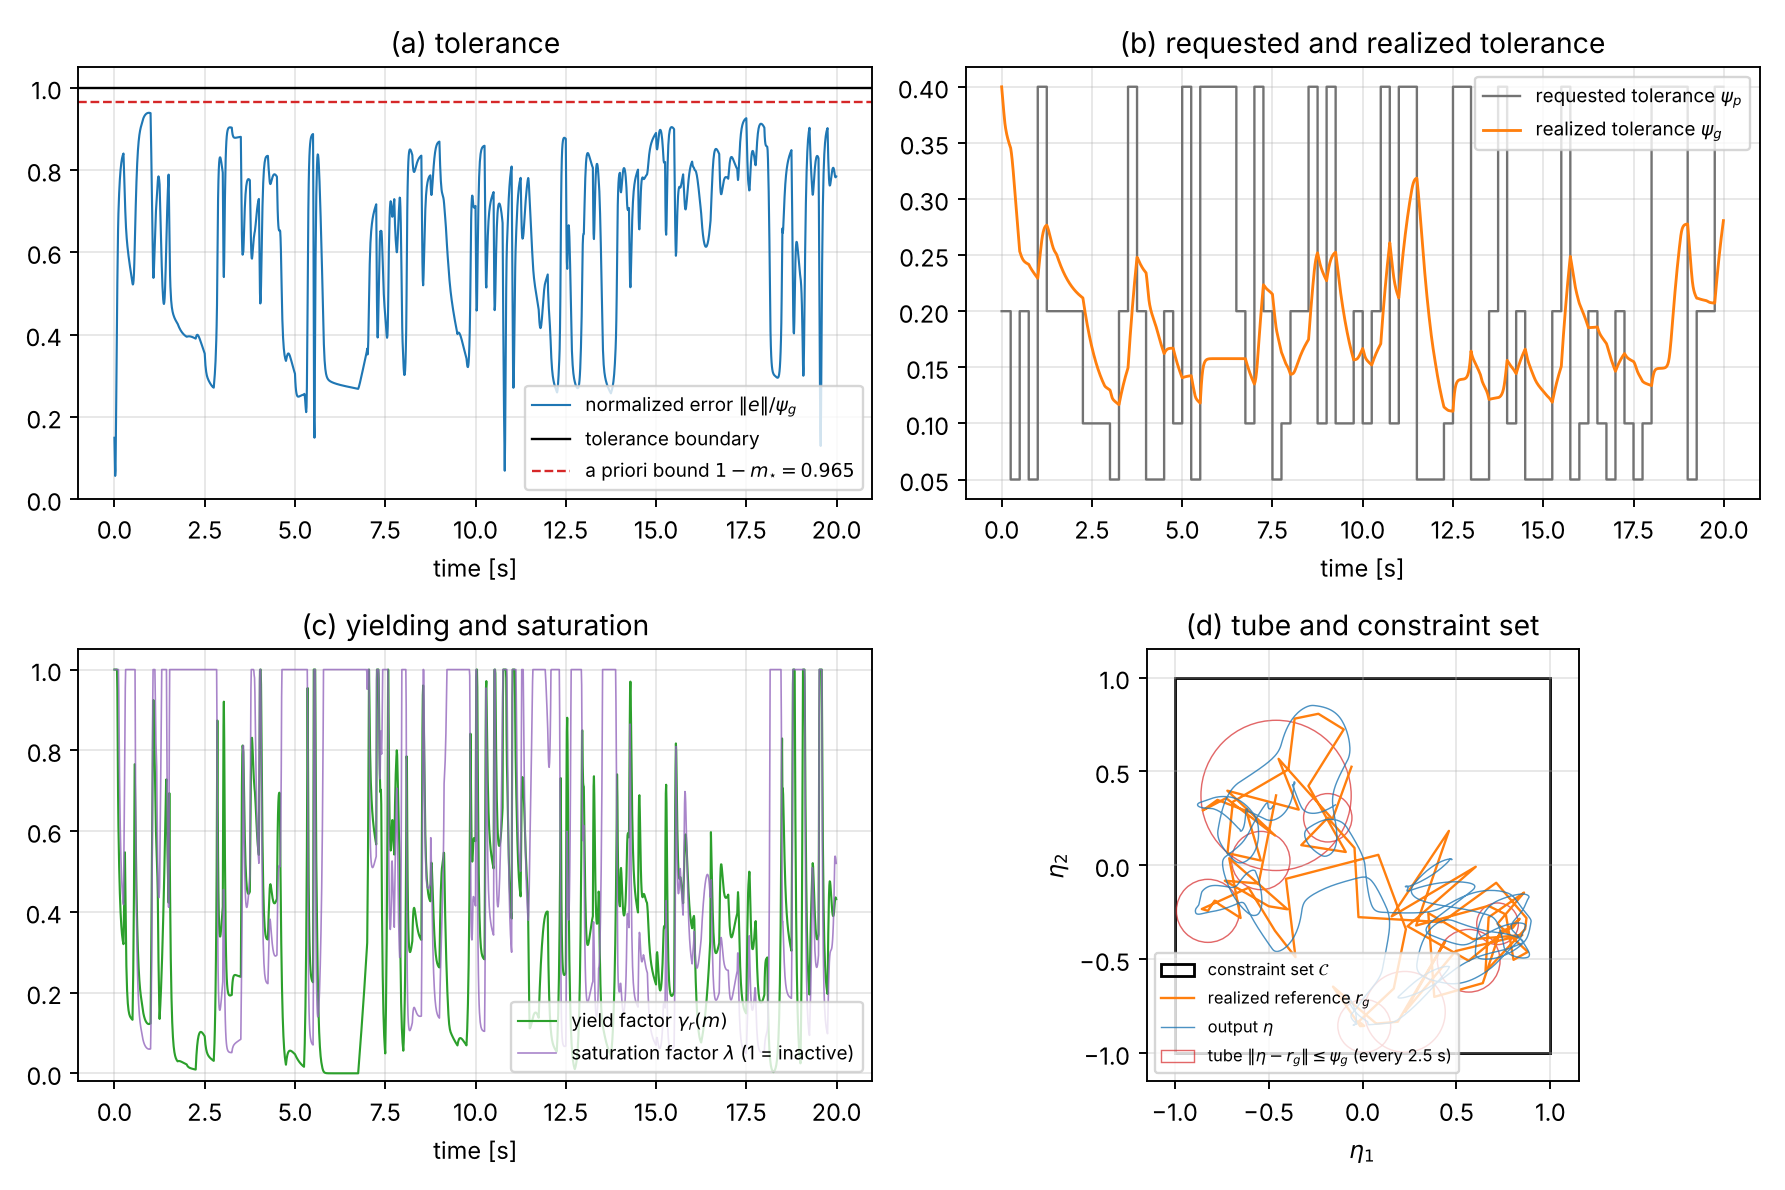
\includegraphics[width=0.98\textwidth]{yield_core.png}
\caption{Closed-loop signals of one case}
\label{fig:trace}
\end{figure}

\section{기존 결과와의 비교}
\label{sec:comp}

비교 대상은 입력 제약 아래에서 허용 오차를 다루는 두 가지 기존 방식이다. Reference 수정은 Verginis가 Fotiadis--Rovithakis의 방법을 가져온 것이라고 밝히고 있으며, 표의 내용은 전문을 읽은 Verginis의 것이다. 확인 수준은 \Cref{app:refs}에 적는다.

\begin{table}[H]
\centering\footnotesize\setlength{\tabcolsep}{4pt}
\caption{Input-constrained tolerance guarantees in the literature and in this note}
\label{tab:comp}
\begin{tabular}{p{3.0cm}p{3.7cm}p{3.6cm}p{3.9cm}}
\toprule
 & 경계의 확장 (Berger) & Reference 수정 (Verginis) & 이 노트 \\
\midrule
입력이 부족할 때 & Saturation 편차에 비례해 funnel 경계를 넓힘 & Saturation 편차로 구동되는 filter가 reference를 이동 & 오차 여유에 따라 reference의 진행과 허용 오차의 수축을 늦춤 \\
Plant 조건 & Sector bound. Input gain의 부호, 내부 동역학의 안정성 불필요 & Input gain의 대칭 부분 양정치, 내부 동역학의 안정성 & (S2)--(S4), authority (C2) 또는 방향별 authority \\
Saturation 수준 & 임의 & 충분히 큼(존재만 보임) & $\rho_0>0$ 또는 $\rho_{\mathrm{dir}}>0$으로 명시 \\
보장되는 것 & 넓어진 funnel 안의 오차, 전역 해. 경계의 상한은 없음 & 수정된 reference에 대한 funnel, 점근 추종 & 고정된 $\Cset$ 안의 output, 사전 상한 $\varepsilon$ \\
상대 차수 & 임의 & 2 이상 & 1, 그리고 기계 system \\
추가 입력 & 없음 & 적분 항 2개 & 크기만 제한된 임의의 feedforward \\
\bottomrule
\end{tabular}
\end{table}

\textbf{가장 가까운 선행 연구.} Das와 Jagtap은 모델을 모르는 Euler--Lagrange system에서 입력 한계 아래 오차 경계를 넓히지 않고 유지하는 명시적 실행 가능 조건을 준다(전문 확인). 실행 가능한 reference에 대해서는 \Cref{prop:mech}와 같은 종류의 보장이 이미 있다. 그들의 조건은 성분별이고, 결합된 관성에서 부호가 섞인 saturation의 경우를 다루지 않는 것으로 보인다(학습 비교 노트에 점 확인이 있다). 이 노트의 방향별 조건은 그 경우를 포함한다.

\textbf{기존 결과가 더 나은 점.} 경계 확장 방식은 authority 조건 없이 임의의 saturation 수준에서 해의 존재를 보장하고, 임의의 상대 차수와 미지의 제어 방향을 다룬다. Reference 수정 방식은 적분 항으로 점근 추종을 얻는다. 이 노트는 상대 차수 1과 기계 system에 한정되고, 수렴은 정확한 표현을 가정한 경우만 다룬다.

\textbf{이 노트가 다른 점.} 경계 확장 방식은 funnel이 bounded임을 일반적으로 보장하지 않으며, bounded임이 증명된 경우는 saturation이 한 번도 작동하지 않을 만큼 수준이 큰 경우이다. 따라서 고정된 제약 집합에 대한 보장으로 쓸 수 없다. Reference 수정 방식의 saturation 조건은 미지의 plant 상수에 의존하는 존재 명제이다. 이 노트의 조건은 class 자료에 대한 명시적 부등식이고 상한 $\varepsilon$은 그로부터 계산되며, 결합된 input gain에 대해 saturation 수준을 키우는 대신 방향 보존 saturation을 쓴다. 또 reference의 속도와 허용 오차가 임의 크기의 외부 명령이며, 학습되는 feedforward가 loop 안에 있어도 보장이 바뀌지 않는다.

\textbf{새로움에 대한 판단.} 경계에서 커지는 feedback, 입력 제약 아래의 reference 수정, 실행 가능한 reference에 대한 명시적 실행 가능 조건은 모두 기존에 있다. 이 노트의 결과 가운데 기존 결과와 다른 것은 방향별 authority 조건과, 임의의 명령에 대해 양보로 보장을 유지한다는 점이다. 후자가 학습에 이득을 주는지는 학습 비교 노트에서 시험했고 지지되지 않았다.

\section{범위와 미해결 항목}
\label{sec:open}

\begin{enumerate}
\item \textbf{조건의 보수성.} (C2)는 가장 약한 방향의 gain $\gamma_0$와 가장 작은 입력 한계 $\bar u_{\min}$의 곱으로 authority를 재며, 7-DOF 수치에서는 성립하지 않는다(\Cref{tab:panda}). \Cref{thm:dir}의 방향별 조건은 성립하지만 그 사전 여유 $m_\star^R$은 작고, \Cref{lem:Rbounds}(a)의 닫힌 형태로 계산하면 더 작다. $R$을 class 자료로부터 인증된 방식으로 계산하는 절차는 만들지 않았다.
\item \textbf{상대 차수 2.} 기계 system은 \Cref{sec:mech}의 output으로 다루며, 위치 제약은 볼록한 집합에 한정된다. 볼록하지 않은 위치 제약, 속도 제약의 직접 지정, 기계 system이 아닌 상대 차수 2는 다루지 않았다.
\item \textbf{진행 보장.} \Cref{thm:main}은 실현된 명령이 제안에 얼마나 가까운지를 말하지 않는다. $\partial\Cset$ 근처에서 \eqref{eq:rg}는 $\partial\Cset$에서 멀어지는 방향의 진행도 늦춘다.
\item \textbf{수렴의 범위.} \Cref{prop:storage}는 isotropic gain, 정확한 표현, saturation이 작동하지 않는 구간에 한정된다. Isotropic이 아닌 input gain에서는 Step 3의 두 항이 상쇄되지 않는다. Saturation이 지속되면 fast weight의 storage가 커지며, 그 경우의 수렴은 다루지 않았다. \Cref{prop:mechstorage}는 isotropic 가정을 없애지만 정확한 표현을 가정한다. 학습된 feature로 표현이 정확하지 않을 때의 결과는 없다.
\item \textbf{Sampled data와 측정 잡음.} 다루지 않았다. 사전 상한 $\varepsilon$이 1에 가까우면 경계 근처의 gain이 크다.
\item \textbf{수치 확인의 범위.} 상대 차수 1, 입력 3개 이하의 점 평가와 입력 2개의 simulation이다. Fast weight의 적응은 isotropic gain과 2-link arm에서 확인했고, 7-DOF arm에서는 authority만 평가했다. RL 학습은 포함하지 않았다.
\end{enumerate}

\appendix

\section{참고문헌과 확인 범위}
\label{app:refs}

\textbf{전문을 읽음.}
\begin{itemize}
\item T. Berger, ``Input-constrained funnel control of nonlinear systems,'' IEEE Transactions on Automatic Control 69(8):5368--5382, 2024, arXiv:2202.05494. 임의의 saturation에서 해의 존재(Theorem 3.1), funnel 경계가 일반적으로 bounded라고 결론지을 수 없다는 저자의 서술, 충분히 큰 saturation 수준에서 saturation이 작동하지 않는다는 결과(Theorem 3.2).
\item T. Berger, ``An improved input-constrained funnel controller for nonlinear systems,'' arXiv:2506.18417, 2025. Funnel 함수 하나를 쓰는 개선.
\item C.~K. Verginis, ``Barrier integral control for global asymptotic tracking of uncertain nonlinear systems under state and input constraints,'' arXiv:2409.04767. Reference 수정과 적분 항(Theorem 2).
\item R. Das, P. Jagtap, ``Prescribed performance control of unknown Euler--Lagrange systems under input constraints,'' arXiv:2507.01426v2. 성분별 실행 가능 조건(식 (11)--(12))과 그 증명.
\item J. Ni, X. Huang, G.~A. Rovithakis, Y. Yan, ``Low-complexity control under input saturation and performance constraints: a bidirectional modification scheme,'' arXiv:2609.00827. Bounded-input bounded-state 가정(Assumption 1)과 그 밖의 경우를 미해결로 둔 서술.
\end{itemize}

\textbf{초록만 확인함.}
\begin{itemize}
\item F. Fotiadis, G.~A. Rovithakis, ``Input-constrained prescribed performance control for high-order MIMO uncertain nonlinear systems via reference modification,'' IEEE Transactions on Automatic Control 69(5):3301--3308, 2024.
\end{itemize}

\textbf{열어 보지 않음.} N. Hopfe, A. Ilchmann, E.~P. Ryan, ``Funnel control with saturation: linear MIMO systems,'' IEEE Transactions on Automatic Control 55(2):532--538, 2010. Berger(2024)의 서론이 이 결과를 충분히 큰 saturation 수준에서의 실행 가능성으로 요약한다.

\end{document}
